\documentclass[12pt,a4paper]{article}
\usepackage[polish]{babel}
\usepackage[T1]{fontenc}
\usepackage{hyperref}
\usepackage{url}
\usepackage{graphicx}
\graphicspath{ {images/} }
\usepackage{csquotes}
\usepackage[utf8x]{inputenc}
\usepackage{fancyvrb}

\addtolength{\hoffset}{-1.5cm}
\addtolength{\marginparwidth}{-1.5cm}
\addtolength{\textwidth}{3cm}
\addtolength{\voffset}{-1cm}
\addtolength{\textheight}{2.5cm}
\setlength{\topmargin}{0cm}
\usepackage{algorithm}
\usepackage[noend]{algpseudocode}
\setlength{\headheight}{0cm}

\begin{document}
    \begin{titlepage}
       \begin{center}
           \vspace*{1cm}
           
           {\fontsize{23}{25}\selectfont Dokumentacja projektu\\BGM-Firebase\\Mobilne interfejsy multimedialne}
            \vspace{0.4cm}
            
            {\fontsize{17}{18}\selectfont Dawid Bitner}
           
            {\fontsize{12}{13}\selectfont 27 marca 2020}
           
            \vfill
            \vspace{0.8cm}
     
            {\fontsize{13}{14}\selectfont Politechnika Śląska\\Wydział Matematyki Stosowanej\\Rok akademicki 2019/2020}
     
       \end{center}
    \end{titlepage}
	\newpage
	\tableofcontents
	\newpage
	\section{Narzędzia, skrypty, źródła zewnętrzne}
	Do realizacji projektu użyłem jako środowiska programistycznego\textit{ Android Studio} w wersji \textit{3.5.1}. \\
    Postanowiłem, że użyję frameworka do języka \textit{Dart} - \textit{Flutter'a} w wersji \textit{v1.12.13+hotfix.8}. \\
	Emulator symulował urządzenie \textit{Nexus 5X}, na którym był zainstalowany system\textit{ Android} w wersji \textit{8.1 API 27}. \\
    \\
    Podczas realizacji projektu użyłem kilku zależności dodanych do projektu we Flutterze - opiszę je krótko na podstawie pliku \textit{pubspec.yaml} \\
    \begin{itemize}
    \begin{verbatim}
dependencies:
  flutter:
    sdk: flutter
  fluttertoast: ^4.0.0
  uuid: 2.0.4
  progress_dialog: ^1.2.2
  # The following adds the Cupertino Icons font to your application.
  # Use with the CupertinoIcons class for iOS style icons.
  cupertino_icons: ^0.1.2
  flutter_simple_dependency_injection: ^1.0.2
  bloc_pattern: ^2.5.1
  provider: ^2.0.1
  rxdart: ^0.23.1
  json_serializable: ^3.2.5
  retrofit: ^1.3.1
  firebase_auth: ^0.16.0
  firebase_database: ^3.1.5
  logger: ^0.8.3


dev_dependencies:
  flutter_test:
    sdk: flutter
  build_runner: ^1.7.4
  retrofit_generator: ^1.3.1+9
    \end{verbatim}
    \end{itemize}
    
    \newpage
    
    \textbf{cupertino-icons} - jest to repozytorium zasobów zawierające domyślny zestaw zasobów ikon używanych przez Flutter - wykorzystałem ikonę lupy do wyszukiwania miasta. \\ \\
    \textbf{retrofit} - wykorzystany w celu łatwego dostępu do API, bez pisania dużej ilości kodu, doskonale współgra z serializatorem i deserializatorem \textit{JSON}. \\ \\
    \textbf{flutter-simple-dependency-injection} - dzięki temu mogłem wykorzystać wstrzykiwanie zależności w swoich programie. \\ \\
    \textbf{json-serializable} - wykorzystany w celu serializacji danych, ułatwia pisanie programu poprzez tworzenie plików, przy użyciu komendy na podstawie prostych zależności zostały stworzone pliki \textit{g.dart} dzięki który można było pobierać dane z API, zarówno dla \textit{Firebase} jak i dla zewnętrznego API do wyszukiwania filmów - w moim przypadku \textit{OMDBApi} które to pobiera dane z bazy filmów \textit{IMDB.com}. Przykład: \\ \\
    plik game.dart:
    \begin{verbatim}
import 'package:firebase_database/firebase_database.dart';
import 'package:json_annotation/json_annotation.dart';

part 'game.g.dart';

@JsonSerializable(explicitToJson: true)
class Game{
  String title;
  String year;
  String genre;
  String studio;
  bool played;
  String id;

  Game({this.title, this.year, this.genre, this.studio, this.played,  this.id});

  void setUuid(String uuid){
    this.id = uuid;
  }

  factory Game.fromJson(Map<String, dynamic> json) => _$GameFromJson(json);
  Map<String, dynamic> toJson() => _$GameToJson(this);

}
    \end{verbatim}
    \newpage
Oraz stworzony na jego podstawie plik game.g.dart:
\begin{verbatim}
// GENERATED CODE - DO NOT MODIFY BY HAND

part of 'game.dart';

// **************************************************************************
// JsonSerializableGenerator
// **************************************************************************

Game _$GameFromJson(Map<String, dynamic> json) {
  return Game(
    title: json['title'] as String,
    year: json['year'] as String,
    genre: json['genre'] as String,
    studio: json['studio'] as String,
    played: json['played'] as bool,
    id: json['id'] as String,
  );
}

Map<String, dynamic> _$GameToJson(Game instance) => <String, dynamic>{
      'title': instance.title,
      'year': instance.year,
      'genre': instance.genre,
      'studio': instance.studio,
      'played': instance.played,
      'id': instance.id,
    };

\end{verbatim}

\textbf{bloc-pattern} - w celu prostszego zastosowania logiki biznesowej w projekcie \\ \\
\textbf{rxdart} - w celu wykorzystania programowania reaktywnego 
\textbf{fluttertoast} - dołączone standardowo - w celu używania wyskakujących powiadomień - \textit{Toastów}. \\ \\
\textbf{intl} - ten pakiet zapewnia funkcje internacjonalizacji i lokalizacji, w tym tłumaczenie wiadomości, liczbę mnogą i płcie, formatowanie i analizę dat / liczb oraz tekst dwukierunkowy. Dołączany standardowo. \\ \\
\textbf{uses-material-design} - w celu używania \textit{Google Design}. \\ \\
\textbf{firebase-auth} i \textbf{firebase-database} - w celu połaczenia się z bazą \textit{Firebase} i autoryzacji użytkownika \textit{Firebase} \\ \\
\textbf{logger} - w celu łatwiejszego i przyjemniejszego dostępu do logów w logcacie.
    
	\section{Problemy podczas realizacji}
Nie miałem większych problemów podczas realizacji tego projektu we Flutterze. Dużą część warstwy widokowej aplikacji posiadałem już zaimplementowaną, ponieważ w poprzednim semestrze realizowałem z innymi osobami projekt na zaliczenie innego przedmiotu bardzo podobny do tego. Do głównych różnic należy zastosowanie \textit{Firebase} jako bazy zdalnej, a nie jak w poprzednim projekcie \textit{SQLite} jako bazy lokalnej, oraz zaimplementowanie modułu zdalnej autoryzacji. Największym problemem okazało się dla mnie dostosowanie wyglądu aplikacji - moim zdaniem stylizacja elementów we Flutterze wymaga dużego nakładu czasowego i jest mało intuicyjne. Posiłkowalem się gotowymi fragmentami kodu znalezionymi w serwisie \textit{medium.com}, dokumentacji, oraz na \textit{stackoverflow}.
    
	\section{Główna część projektu}
Jako stronę powitalną mamy do użytku element z dynamiczną zakładką, dzięki któremu możemy się zarejestrować w naszej bazie, bądź też zalogować na już istniejące konto.: \\
    \begin{center}
        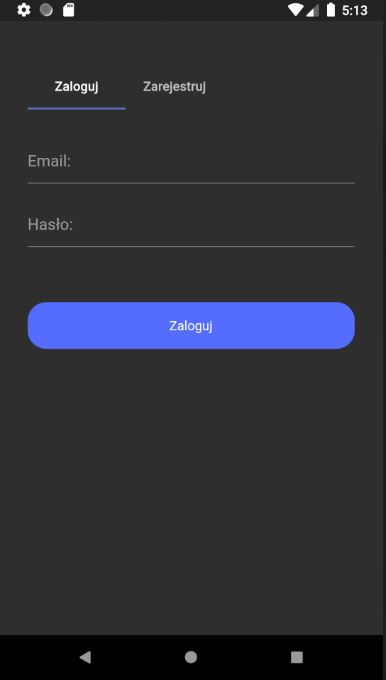
\includegraphics[scale=0.70]{1.JPG}
        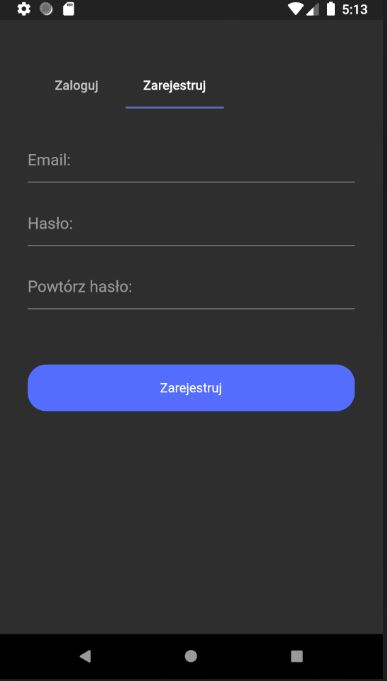
\includegraphics[scale=0.70]{2.JPG}
            \begin{scriptsize}
            \\ Zakładki logowania i rejestracji
            \end{scriptsize}
    \end{center}
    
    Po zarejestrowaniu, gdzie sprawdzana jest poprawność adresu e-mail, długość hasła, oraz poprawność powtórzenia, zostaniemy przeniesieni do naszego pustego obszaru, analogicznie po zalogowaniu się już na istniejące konto zostaniemy przeniesieni do obszaru, gdzie znajdują się nasze gry, filmy oraz książki. \\
    \begin{center}
        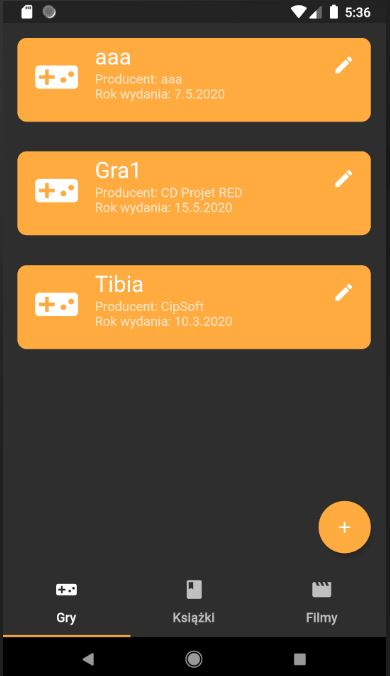
\includegraphics[scale=0.70]{3.JPG}
        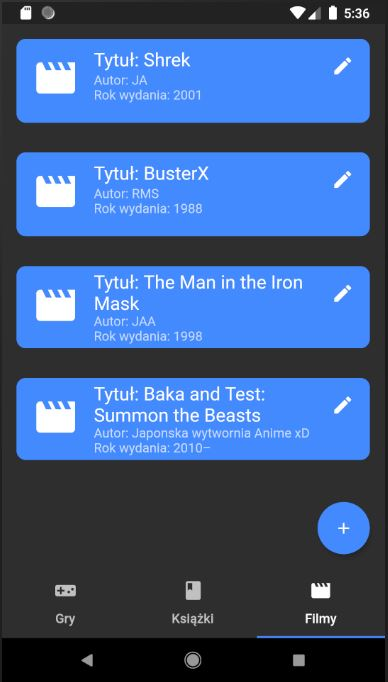
\includegraphics[scale=0.70]{4.JPG}
            \begin{scriptsize}
            \\ Zakładka gier i filmów
            \end{scriptsize}
    \end{center}
    Klikając plus, na zakładce książek i gier, możemy dodać interesujące nas tytuły ręcznie, natomiast klikając plus w zakładce filmów przechodzimy do widgetu z wyszukiwarką filmów w \textit{OMDB Api}
    \begin{center}
        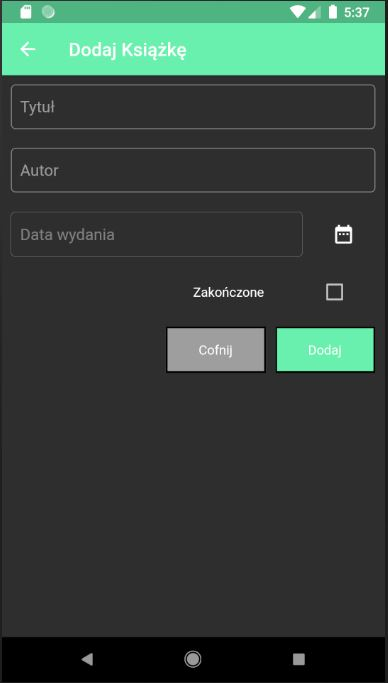
\includegraphics[scale=0.70]{5.JPG}
        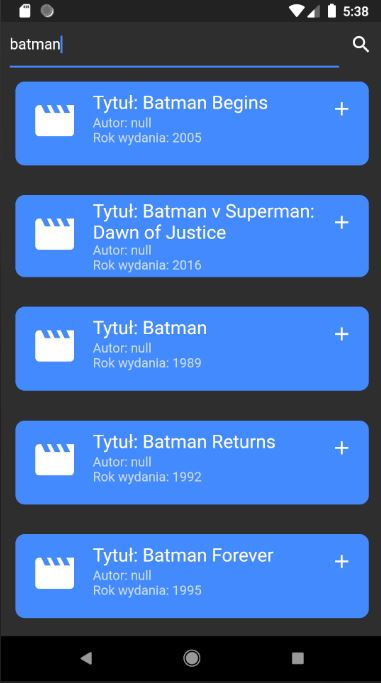
\includegraphics[scale=0.70]{6.JPG}
            \begin{scriptsize}
            \\ Zakładka gier i filmów
            \end{scriptsize}
    \end{center}
    Dodane już elementy do naszej bazy możemy usuwać i edytować. Możemy usunąć przesuwając taki element na liście w prawo, bądź klikając w edycję, a następnie usunąć poprzez dotknięcie ikony śmietnika, gdzie naturalnie możemy także dokonywać zmian w bazie. Poprzez \textit{OMDB Api} nie jest pobierany reżyser filmu, więc w takim przypadku musimy go dodać ręcznie.
    \begin{center}
        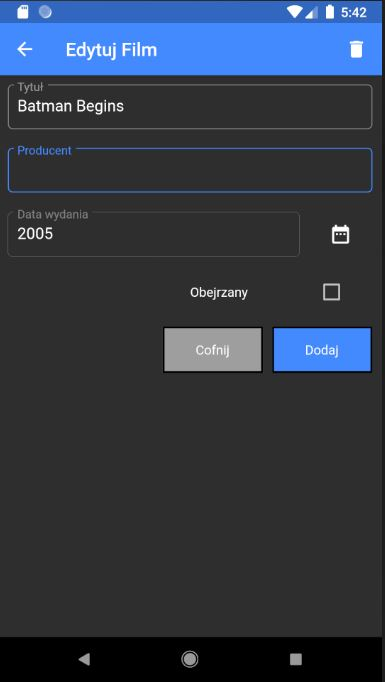
\includegraphics[scale=0.70]{7.JPG}
        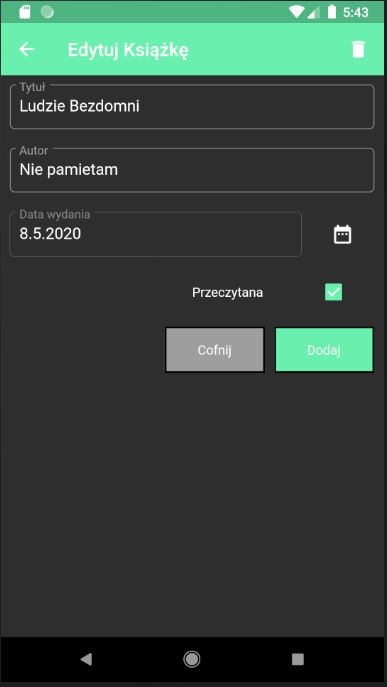
\includegraphics[scale=0.70]{8.JPG}
            \begin{scriptsize}
            \\ Zakładka gier i filmów
            \end{scriptsize}
    \end{center}
    
	\section{Opinia}
Próbowałem stworzyć aplikację która będzie przyjazna dla użytkownika - przede wszystkim w działaniu i wizualnie, zastosowałem proste widgety, komponenty. Aplikacja oferuje pełen CRUD na bazie Firebase. W mojej opinii jest dobrą podstawą pod rozbudowę i stworzenie bardzo zaawansowanego systemu do zarządzania rekordami w bazie za pomocą Fluttera i Firebase.

W repozytorium znajduje się kalendarium prac, dokumentacja, pliki projektu, oraz film prezentujący.
https://github.com/dawbit/flutter-firebase

\end{document}
